\documentclass[journal,onecolumn,11pt,a4paper,draftclsnofoot]{IEEEtran}
\IEEEoverridecommandlockouts

% ACS citation style (achemso.sty, achemso.bst and natmove.sty are in this folder).
% The class option list is hidden while it loads, because achemso reads the
% IEEEtran option `journal' as its own key.
\makeatletter
\let\zk@classopts\@classoptionslist
\let\@classoptionslist\@empty
\usepackage[articletitle=true,super=true]{achemso}
\let\@classoptionslist\zk@classopts
% ACS numbers the reference list as (1), (2), ...
\def\@biblabel#1{(#1)}
\makeatother
\usepackage{amsmath,amssymb,amsfonts}
\usepackage{graphicx}
\usepackage{textcomp}
\usepackage{xcolor}
\usepackage{booktabs}
\usepackage{tabularx}
\usepackage{microtype}
\usepackage{tikz}
\usetikzlibrary{arrows.meta,positioning}
\usepackage[hyphens]{url}
\usepackage{hyperref}

\hypersetup{
    colorlinks=true,
    linkcolor=blue,
    citecolor=blue,
    urlcolor=blue
}

\renewcommand{\UrlBreaks}{\do\/\do\-\do\_\do\.}
\newcommand{\co}{CO$_2$}
\newcommand{\xco}{x_{\mathrm{CO_2}}}
\newcommand{\tbc}[1]{\textcolor{red}{[#1]}}

\begin{document}

\title{Machine-Learning Prediction of CO$_2$ Solubility in Ionic Liquids from DFT Ion Descriptors}

\author{Maulana~Ragil~Zakariah}

\markboth{}%
{Zakariah: ML Prediction of CO$_2$ Solubility in Ionic Liquids}

\maketitle

\begin{abstract}
Ionic liquids (ILs) are candidate solvents for \co{} capture, but measuring \co{} solubility for every possible cation--anion pair is not feasible. This work presents a workflow that predicts \co{} solubility in ILs from quantum-chemical descriptors of the individual ions. An experimental dataset of 11,256 solubility points for 113 ILs (50 cations, 26 anions) covers 243--453~K and up to 50~MPa. Each ion was converted from its name to a SMILES string and then to a 3D structure with RDKit, and optimised with r2SCAN-3c in ORCA 6.0. Five descriptors per ion were extracted: total energy, HOMO and LUMO energies, HOMO--LUMO gap and dipole moment. Together with temperature, pressure and elemental atom counts they give 248 input features. Four regressors were trained on a random 80/20 split. Random Forest gave the best test-set performance ($R^2 = 0.985$, MAE $= 0.017$ in mole fraction), followed by Gradient Boosting (0.973), a neural network (0.966) and Ridge regression (0.591). Permutation importance ranks pressure first, temperature second and the anion total energy third. The trained model was used to screen 25 imidazolium ILs and to make first predictions for two bio-based ILs, [BMIM][oleate] and [BMIM][laurate]. The dataset was also rebuilt from NIST ILThermo with full source references (12,297 points, 160 publications). A check of the workflow found issues that affect the reported results: errors in the descriptor extraction, a validation split that lets the same IL appear in both training and test sets, and inconsistent inputs for the bio-based ILs. These are documented in Section~\ref{sec:issues}, together with grouped cross-validation results that give a more realistic estimate of performance on unseen ILs.
\end{abstract}

\begin{IEEEkeywords}
Ionic liquids, CO$_2$ capture, solubility prediction, machine learning, density functional theory, r2SCAN-3c, Random Forest.
\end{IEEEkeywords}

\section{Introduction}
\label{sec:intro}

Ionic liquids (ILs) are salts that are liquid below about 100\,\textdegree C. Their negligible vapour pressure, thermal stability and the freedom to pair many cations with many anions make them candidate solvents for \co{} capture \cite{blanchard1999green, brennecke2010ionic, zhang2012carbon, aghaie2018systematic}. In common imidazolium ILs, \co{} dissolves mainly by physical absorption, and the anion has the largest effect on solubility \cite{cadena2004why, anthony2005anion}. Functionalised ILs can also bind \co{} chemically \cite{bates2002co2, gurkan2010equimolar}. The number of possible cation--anion pairs is very large, while each solubility isotherm requires dedicated high-pressure measurements. A model that predicts solubility for ILs that have not been measured would let experiments focus on the most promising candidates.

Data-driven models have been built for this task, from early neural networks \cite{eslamimanesh2011artificial} to tree ensembles and deep networks trained on several thousand points \cite{venkatraman2017predicting, song2020prediction, ali2024prediction}. Most use group-contribution or COSMO-derived inputs. This work instead describes each ion with a small set of descriptors computed by density functional theory (DFT), so that any ion whose structure is known can be described without experimental input. A further motivation is local: Indonesia is a major producer of palm and coconut oil, whose fatty acids (oleic and lauric acid) could supply the anions of bio-based ILs.

The contributions of this work are:
\begin{enumerate}
    \item an experimental dataset of 11,256 \co{} solubility points for 113 ILs, and a rebuilt version with full source references (Section~\ref{sec:data});
    \item a pipeline from ion names to SMILES, 3D structures and r2SCAN-3c calculations, giving five DFT descriptors per ion (Section~\ref{sec:comp});
    \item a comparison of four regressors and a feature-importance analysis (Sections~\ref{sec:models} and~\ref{sec:results});
    \item a first screening of imidazolium ILs and of two bio-based ILs (Section~\ref{sec:screening}).
\end{enumerate}
Section~\ref{sec:issues} reports the limitations found when the workflow was checked against the raw calculation outputs, and Section~\ref{sec:summary} concludes.

\section{Experimental Data}
\label{sec:data}

\subsection{Training dataset}
The training data come from two tables of the Supporting Information of Laakso et al.\cite{laakso2025machine} (\path{data/raw/rawdata.xlsx}), whose experimental data were compiled by Song et al.\cite{song2020prediction} (10,116 points for 124 ILs). Table S6 is that compilation, with pressure in bar together with fugacities and UNIFAC activity coefficients; Table S5 is the 1,889-point test set of Laakso et al., taken from the same compilation after removal of duplicates and given with pressure in kPa. Only $T$, $P$ and the \co{} mole fraction $\xco$ were kept. Pressures were converted to kPa and the two tables were concatenated into 12,005 points (\path{notebooks/thesis/02-data-preprocessing.ipynb}). Because Table S5 is a subset of Table S6, and Table S6 itself contains repeated points, the result contains duplicates (Section~\ref{sec:issues}).

Each IL is identified by a cation and an anion abbreviation. The abbreviations were mapped to full ion names (84 unique ions). After merging with the DFT descriptors (Section~\ref{sec:comp}), points whose ions had no successful calculation were dropped. This left the thesis training set of 11,256 points (\path{data/thesis/final_model_dataset_v3.csv}), of which 2,013 are exact repeats of an earlier row (9,243 distinct points). Neither source table gives a reference for each point. Matching against the referenced dataset below traces 8,778 of the 11,256 points (78\%) to one of 106 publications (\path{data/thesis/thesis_point_references.csv}). It is summarised in Table~\ref{tab:dataset} and Fig.~\ref{fig:dataset}; it is dominated by imidazolium cations, and the number of points per IL is uneven, from 1 to 871.

\begin{table}[t]
\caption{The thesis training set (used for the random-split comparison in Table~\ref{tab:metrics}) and the referenced dataset (used for the grouped-validation results in Table~\ref{tab:grouped}).}
\label{tab:dataset}
\centering
\begin{tabular}{lcc}
\toprule
 & \textbf{Thesis set (v3)} & \textbf{Referenced set} \\
\midrule
Data points & 11,256 & 12,297 \\
Ionic liquids & 113 & 109 \\
Cations / anions & 50 / 26 & 39 / 22 \\
Temperature (K) & 243.2--453.2 & 228.2--450.5 \\
Pressure & 0.8~kPa--50.0~MPa & 0.1~kPa--99.0~MPa \\
$\xco$ & 0.00006--0.952 & 0.000004--0.9999 \\
Points per IL (median) & 52 & 68 \\
Source references & Song et al.\cite{song2020prediction} (78\% traced) & 171 publications, DOIs verified \\
Measurement method per point & no & yes \\
\bottomrule
\end{tabular}
\end{table}

\begin{figure}[t]
\centering
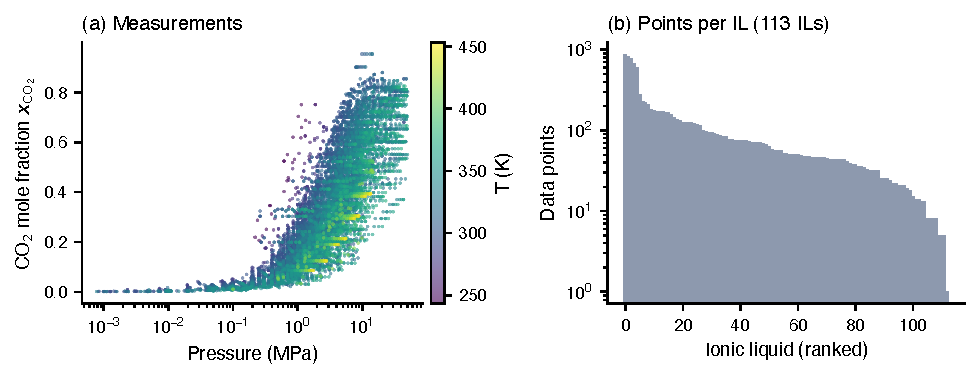
\includegraphics[width=0.9\textwidth]{figures/fig_dataset.pdf}
\caption{Training dataset. (a) \co{} mole fraction against pressure, coloured by temperature. (b) Number of data points for each of the 113 ILs, ranked.}
\label{fig:dataset}
\end{figure}

\subsection{Referenced dataset}
Because the per-point sources were not recorded in the original tables, the dataset was rebuilt from NIST ILThermo\cite{dong2007ilthermo}. The rebuild was restricted to ILs whose cation and anion both have DFT descriptors (\path{scripts/build_referenced_dataset.py}). Molality and mass-fraction data were converted to mole fraction using molar masses computed from the SMILES strings, and exact duplicates were removed. The result has 12,297 points for 109 ILs from 171 publications (2001--2025: 169 journal articles, one book chapter and one PhD thesis). Each point carries the citation, DOI and experimental method. The citations come from ILThermo, but the DOIs were first added from the top hit of a bibliographic search without a check. All 171 were therefore verified against the Crossref record of each publication (title, year, first author and volume; \path{scripts/verify_dataset_references.py}). In 33 publications (2,218 points) the DOI belonged to a different work and in 18 (2,510 points) to a Supporting Information file; 77 points had no DOI. All were corrected, and the outcome of the check for each publication is in \path{data/references/doi_verification.csv}. Static closed-cell measurements make up 35\% of the points and gravimetric methods about 20\%; static closed-cell measurements make up 35\% of the points and gravimetric methods about 20\%. The bibliography is in \path{data/references/dataset_references.bib}. Merged with the corrected descriptors, it gives the model table \path{data/processed/final_referenced_model_dataset_r2scan3c.csv}, which is the basis of the main results (Section~\ref{sec:results}). It is dominated by [Tf$_2$N]$^-$ (4,126 points) and imidazolium cations (82\% of the points).

\section{Computational Methods}
\label{sec:comp}

Fig.~\ref{fig:pipeline} summarises the workflow from ion names to model inputs.

\begin{figure}[t]
\centering
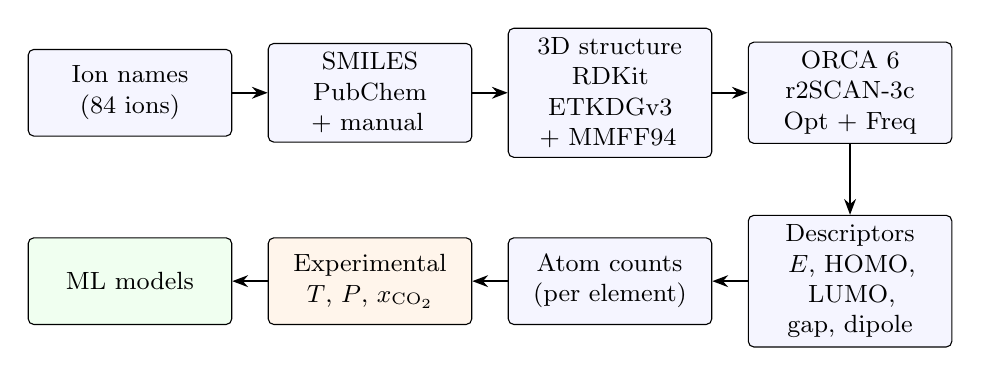
\begin{tikzpicture}[
  box/.style={draw, rounded corners=2pt, align=center, font=\small, minimum height=1.1cm, text width=2.35cm, fill=blue!4},
  dat/.style={box, fill=orange!8},
  arr/.style={-{Stealth[length=2mm]}, thick}]
\node[box] (names) {Ion names\\(84 ions)};
\node[box, right=0.45cm of names] (smiles) {SMILES\\PubChem + manual};
\node[box, right=0.45cm of smiles] (geom) {3D structure\\RDKit ETKDGv3\\+ MMFF94};
\node[box, right=0.45cm of geom] (dft) {ORCA 6\\r2SCAN-3c\\Opt + Freq};
\node[box, below=0.9cm of dft] (desc) {Descriptors\\$E$, HOMO, LUMO,\\gap, dipole};
\node[box, left=0.45cm of desc] (counts) {Atom counts\\(per element)};
\node[dat, left=0.45cm of counts] (exp) {Experimental\\$T$, $P$, $\xco$};
\node[box, left=0.45cm of exp, fill=green!6] (ml) {ML models};
\draw[arr] (names) -- (smiles);
\draw[arr] (smiles) -- (geom);
\draw[arr] (geom) -- (dft);
\draw[arr] (dft) -- (desc);
\draw[arr] (desc) -- (counts);
\draw[arr] (counts) -- (exp);
\draw[arr] (exp) -- (ml);
\end{tikzpicture}
\caption{Workflow from ion names to the model input. Descriptors are computed for each isolated ion and joined to the experimental points by cation and anion.}
\label{fig:pipeline}
\end{figure}

\subsection{Structures}
SMILES strings for the 84 ions were retrieved from PubChem\cite{kim2023pubchem} by ion name; ions that PubChem did not resolve were entered by hand (\path{data/ions/ions_with_smiles.csv}). Every SMILES was checked to describe a single fragment with formal charge $+1$ (cations) or $-1$ (anions) and an even number of electrons; six that described a neutral molecule or an ion together with its counter-ion were corrected (Section~\ref{sec:issues}). Three-dimensional structures were generated with RDKit\cite{rdkit} using the ETKDGv3 embedding\cite{wang2020improving}, followed by an MMFF94 force-field optimisation\cite{halgren1996mmff}. One conformer was generated per ion. Structures are stored in \path{calculations/structures/}.

\subsection{DFT calculations}
Each ion was calculated in isolation in the gas phase with ORCA\cite{neese2022orca}. The method was the r2SCAN-3c composite\cite{grimme2021r2scan}, with a geometry optimisation followed by a frequency calculation (\texttt{! r2SCAN-3c Opt Freq}). Charges were $+1$ for cations and $-1$ for anions, with singlet multiplicity. Outputs are in \path{calculations/ions/}.

Most ions were calculated with ORCA 6.0.0. Nine ions were recalculated with ORCA 6.1.1: the six built from wrong SMILES, [PF$_6$]$^-$, whose original optimisation dissociated into PF$_5$ + F$^-$, and [HSO$_4$]$^-$ and [C$_3$F$_7$CO$_2$]$^-$, whose original structures had one imaginary frequency (Section~\ref{sec:issues}). [PF$_6$]$^-$ was restarted from an ideal octahedron, [HSO$_4$]$^-$ from its previous geometry with the O--H bond rotated by 60\textdegree, and [C$_3$F$_7$CO$_2$]$^-$ with tighter convergence criteria and a finer integration grid (\texttt{TightOpt}, \texttt{DefGrid3}). To check that the two program versions are interchangeable, [BMIM]$^+$ was recalculated with 6.1.1 from the same starting structure: the final energy agrees to $10^{-8}$~Hartree and the HOMO energy is identical. On macOS, the analytic r2SCAN-3c frequency calculation of ORCA 6.1.1 failed for ions above about 30 atoms; for these ([HMMIM]$^+$, [P$_{4,4,4,4}$]$^+$ and [C$_{12}$PhSO$_3$]$^-$) the frequencies were computed on the optimised geometry on the BRIN Mahameru cluster. All 76 ions of the thesis training set and all 61 ions of the referenced training set are true minima with no imaginary frequencies.

\subsection{Descriptors}
Five properties were taken from each ion's output at the optimised geometry:
\begin{itemize}
    \item total electronic energy $E$ (Hartree);
    \item energy of the highest occupied molecular orbital, $E_{\mathrm{HOMO}}$ (Hartree);
    \item energy of the lowest unoccupied molecular orbital, $E_{\mathrm{LUMO}}$ (Hartree);
    \item HOMO--LUMO gap, $E_{\mathrm{LUMO}} - E_{\mathrm{HOMO}}$;
    \item magnitude of the dipole moment (Debye), taken with ORCA's default origin.
\end{itemize}
They were extracted with \path{scripts/extract_descriptors.py}, which reads the last energy, the last orbital-energy block and the dipole magnitude, and records convergence and the number of imaginary frequencies for each ion (\path{data/processed/dft_descriptors_r2scan3c.csv}). The parser used for the original thesis models read some of these values from the wrong part of the output (Section~\ref{sec:issues}); both descriptor sets are compared in Section~\ref{sec:results}. Elemental atom counts were added for each ion, one column per element of the periodic table, of which 15 are non-zero for at least one ion (B, C, F, H, N, O, P and S in anions; C, F, H, N, O, P and S in cations). The descriptors of the cation and the anion were joined to every experimental point of the corresponding IL.

\subsection{Check of the descriptors against published values}
\label{sec:desc-check}
Absolute orbital energies from different methods are not directly comparable, so the descriptors were checked on their ordering. The anion and cation $-E_{\mathrm{HOMO}}$ values were compared with ionisation energies of the same ions computed at the B3LYP-D3(BJ)/6-311+G(d,p) level in an ionic-liquid-like continuum and aligned to valence photoelectron spectra\cite{fogarty2025dos}, and the HOMO--LUMO gaps with PBE-D3(BJ)/DZP gaps from an open ionic-liquid database\cite{stavarache2026xtb}. With the corrected descriptors the Spearman rank correlation is 0.82 for the 14 anions in common and 0.77 for the 9 cations; for the gaps it is 0.94 (6 anions) and 0.98 (13 cations). The HOMO energies used in the thesis models have a rank correlation of $-0.25$ with the published anion ionisation energies (\path{scripts/check_descriptors_vs_literature.py}). The remaining disagreement for anions, for example [TCB]$^-$ ranked too high and [BF$_4$]$^-$ too low, is consistent with the lack of diffuse functions in the r2SCAN-3c basis set, which affects gas-phase anion orbital energies.

\section{Machine-Learning Models and Validation}
\label{sec:models}

\subsection{Thesis protocol: random split}
In the original thesis work, four regressors were trained on the thesis set with the thesis descriptors (248 feature columns: temperature, pressure, 10 DFT descriptors and 236 atom-count columns):
\begin{itemize}
    \item \textbf{Ridge regression}\cite{hoerl1970ridge} with $\alpha = 1$, as a linear baseline;
    \item \textbf{Random Forest}\cite{breiman2001random} with 100 trees;
    \item \textbf{Gradient Boosting}\cite{friedman2001greedy} with 100 trees;
    \item \textbf{a neural network}: a fully connected network with hidden layers of 128, 64 and 32 ReLU units and dropout of 0.2 after the second layer, trained with Adam\cite{kingma2015adam} on mean squared error for 100 epochs with a batch size of 32, in Keras\cite{chollet2015keras}.
\end{itemize}
The first three use scikit-learn\cite{pedregosa2011scikit} with default settings apart from those listed. The dataset was split at random into 80\% training (9,004 points) and 20\% test (2,252 points) with a fixed seed, and features were standardised with a scaler fitted on the training set (\path{notebooks/thesis/17-final-model-comparison.ipynb}). These results are reported for comparison with the thesis only, because a random split of points does not measure prediction for new ILs (Section~\ref{sec:grouped}).

\subsection{Main protocol: grouped cross-validation}
\label{sec:grouped-method}
A typical IL contributes tens to hundreds of points along a few isotherms. With a random split, almost every test point has neighbours from the same IL, and often the same isotherm, in the training set, so the test score measures interpolation along a known isotherm. The main results therefore use the curated dataset (Section~\ref{sec:curated}) and four 5-fold cross-validation schemes that differ in what is held out together\cite{meredig2018can, cawley2010overfitting}:
\begin{itemize}
    \item \textbf{point-wise}: random points, as in the thesis protocol;
    \item \textbf{leave-IL-out}: all points of an IL;
    \item \textbf{leave-cation-out}: all ILs that share a cation;
    \item \textbf{leave-anion-out}: all ILs that share an anion.
\end{itemize}
Leave-anion-out is the most demanding test and the most relevant one, because the anion controls physical \co{} solubility most strongly\cite{cadena2004why, anthony2005anion} and a screening study would vary the anion. The folds are identical for every feature set and model, so differences between feature sets are not due to different splits. $R^2$ and the mean absolute error (MAE, in mole fraction) are reported as the mean and standard deviation over the five folds.

Two tree ensembles were used: a Random Forest with 300 trees and a histogram-based gradient-boosting model\cite{ke2017lightgbm} (scikit-learn \texttt{HistGradientBoostingRegressor}, 500 iterations, learning rate 0.05). Six feature sets were compared, all with temperature and pressure ($T$, $P$):
\begin{itemize}
    \item $T$, $P$ only;
    \item $T$, $P$ and the 15 varying atom counts, counted from the optimised ion structures (ion identity and size, no quantum chemistry);
    \item $T$, $P$ and the 10 thesis DFT descriptors;
    \item $T$, $P$ and the 10 corrected DFT descriptors;
    \item each of the two DFT sets together with the atom counts.
\end{itemize}
The analysis is in \path{scripts/compare_descriptor_sets.py}; per-anion errors of the leave-anion-out predictions are stored with the results in \path{paper/data/}.

\section{Results}
\label{sec:results}

\subsection{Thesis protocol: random split}
Table~\ref{tab:metrics} and Fig.~\ref{fig:parity} show the test-set performance of the thesis models on the random 80/20 split. The three non-linear models reach $R^2 > 0.96$, with Random Forest best on every metric. Ridge regression fails at high solubility, where the dependence on pressure is strongly non-linear. These numbers use the thesis descriptors and a split in which nearly every test IL is also in the training set, and 29\% of the test points have an identical copy in the training set (Section~\ref{sec:issues}); Section~\ref{sec:grouped} shows that they overstate the accuracy for new ILs.

\begin{table}[t]
\caption{Thesis protocol: test-set performance of the four models on the thesis set with the thesis descriptors (random 80/20 split, 2,252 test points). MAE and RMSE are in mole fraction. Training times are for one fit on a laptop CPU.}
\label{tab:metrics}
\centering
\begin{tabular}{lcccc}
\toprule
\textbf{Model} & $R^2$ & \textbf{MAE} & \textbf{RMSE} & \textbf{Training time (s)} \\
\midrule
Random Forest & 0.9853 & 0.0167 & 0.0275 & 1.0 \\
Gradient Boosting & 0.9729 & 0.0257 & 0.0374 & 1.1 \\
Neural network & 0.9656 & 0.0346 & 0.0422 & 19.7 \\
Ridge regression & 0.5906 & 0.1164 & 0.1455 & 0.1 \\
\bottomrule
\end{tabular}
\end{table}

\begin{figure}[t]
\centering
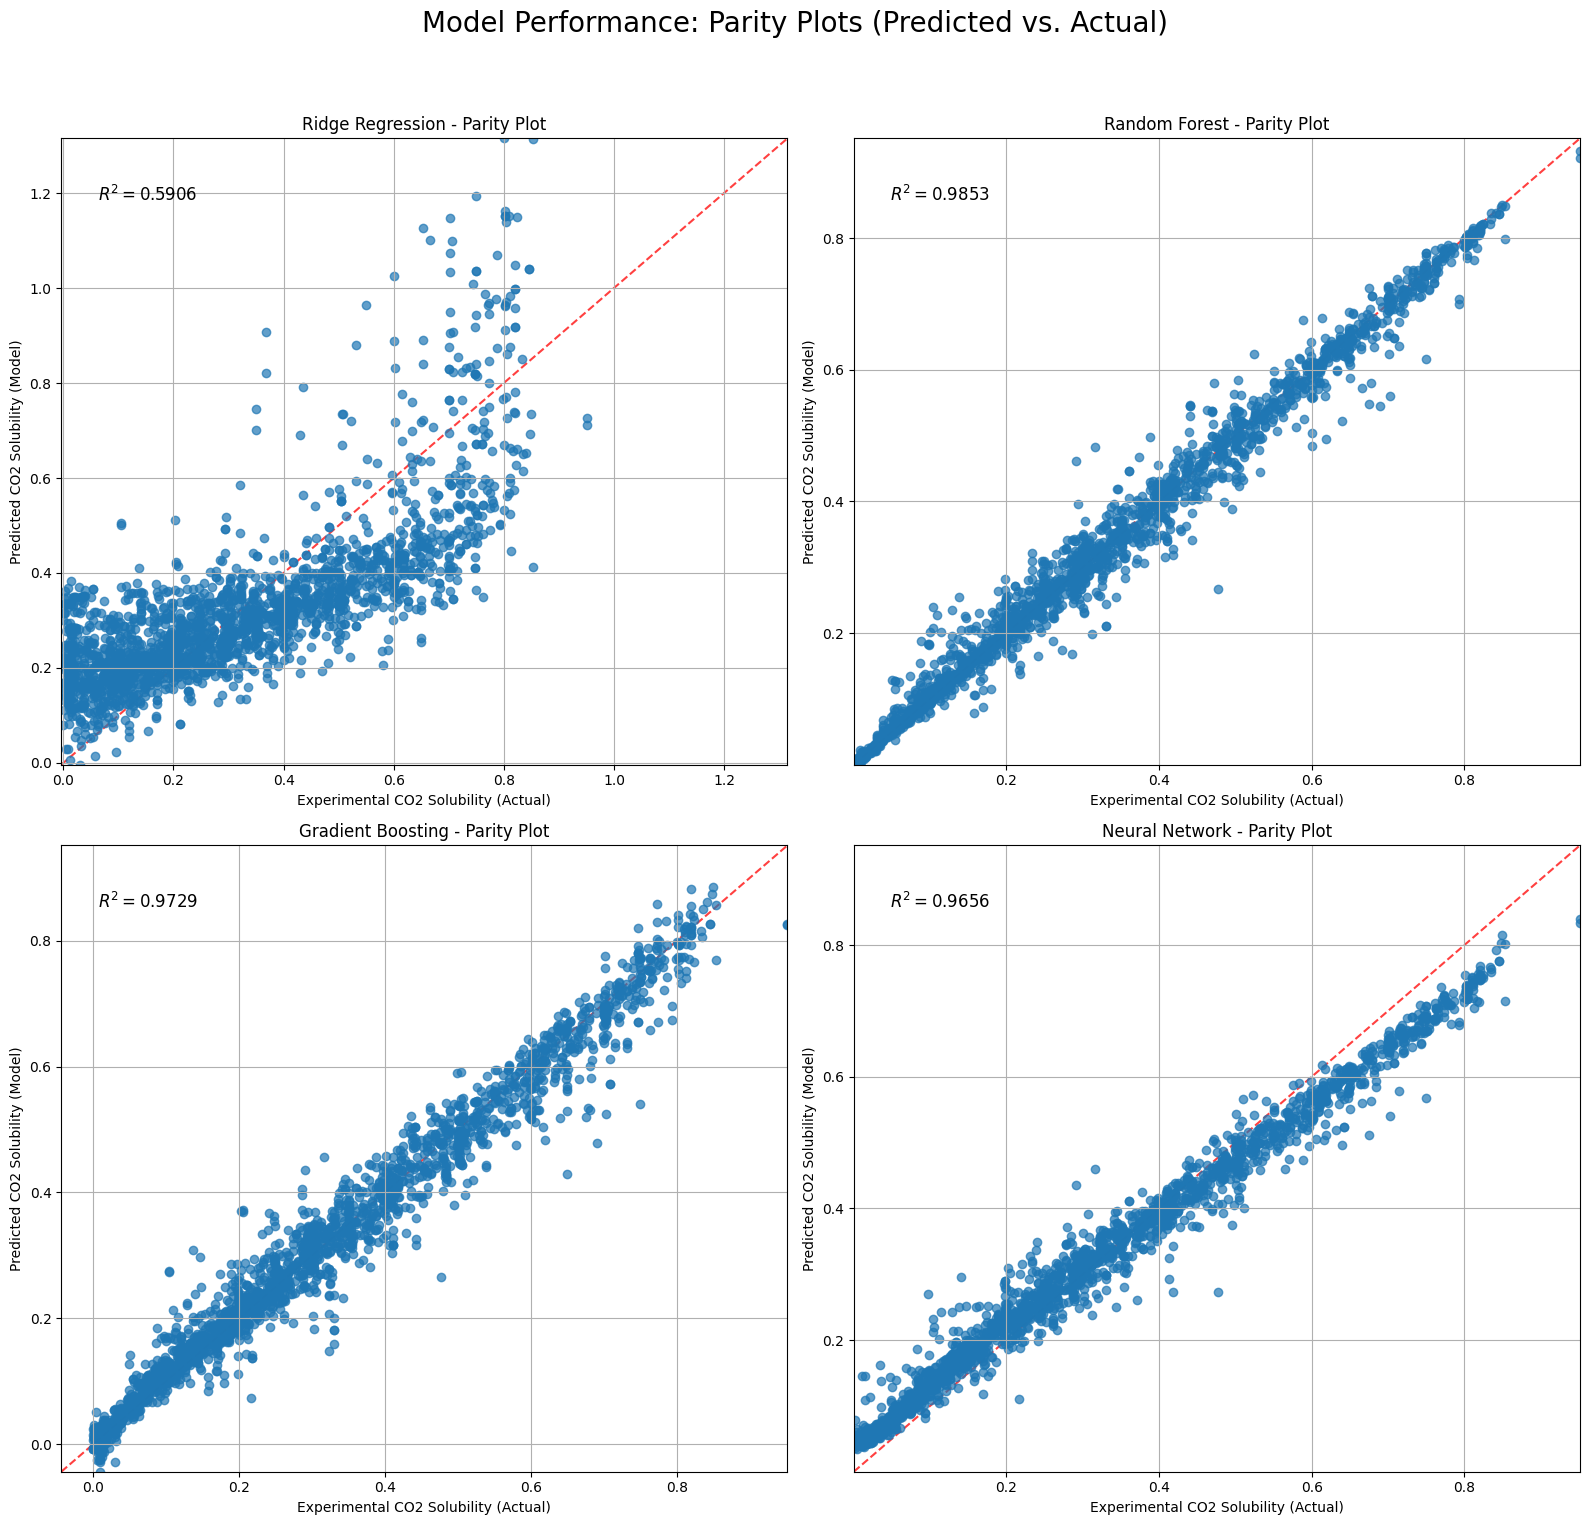
\includegraphics[width=0.8\textwidth]{figures/fig_parity_thesis.png}
\caption{Thesis protocol: predicted against experimental \co{} solubility on the random test set for the four models. The dashed line marks perfect agreement.}
\label{fig:parity}
\end{figure}

\subsection{Grouped validation and descriptor comparison}
\label{sec:grouped}
Table~\ref{tab:grouped} and Fig.~\ref{fig:grouped} give the results of the main protocol on the curated dataset. Four observations stand out.

\begin{table}[t]
\caption{Main protocol: 5-fold cross-validation on the curated dataset (12,026 points, 110 ILs). $R^2$ is the mean $\pm$ standard deviation over the folds; MAE (mole fraction) is the fold mean for leave-anion-out. RF: Random Forest; GB: histogram gradient boosting. Counts: elemental atom counts.}
\label{tab:grouped}
\centering
\small
\setlength{\tabcolsep}{5pt}
\begin{tabular}{llcccc}
\toprule
 & & \multicolumn{3}{c}{\textbf{$R^2$}} & \textbf{MAE} \\
\cmidrule(lr){3-5} \cmidrule(lr){6-6}
 & \textbf{Features ($T$, $P$ +)} & \textbf{Point-wise} & \textbf{Leave-IL-out} & \textbf{Leave-anion-out} & \textbf{Leave-anion-out} \\
\midrule
RF & --- & 0.848 & $0.833 \pm 0.033$ & $0.773 \pm 0.062$ & 0.075 \\
 & counts & 0.982 & $0.953 \pm 0.014$ & $0.873 \pm 0.030$ & 0.054 \\
 & thesis DFT & 0.981 & $0.951 \pm 0.011$ & $0.841 \pm 0.109$ & 0.055 \\
 & corrected DFT & 0.983 & $0.953 \pm 0.018$ & $\mathbf{0.896 \pm 0.016}$ & 0.052 \\
 & thesis DFT + counts & 0.983 & $0.955 \pm 0.013$ & $0.843 \pm 0.111$ & 0.057 \\
 & corrected DFT + counts & 0.983 & $0.955 \pm 0.015$ & $0.890 \pm 0.019$ & 0.053 \\
\midrule
GB & --- & 0.871 & $0.854 \pm 0.028$ & $0.801 \pm 0.058$ & 0.071 \\
 & counts & 0.990 & $0.968 \pm 0.008$ & $0.906 \pm 0.026$ & 0.047 \\
 & thesis DFT & 0.990 & $0.959 \pm 0.018$ & $0.887 \pm 0.073$ & 0.046 \\
 & corrected DFT & 0.990 & $0.960 \pm 0.017$ & $\mathbf{0.925 \pm 0.018}$ & 0.043 \\
 & thesis DFT + counts & 0.990 & $0.968 \pm 0.009$ & $0.884 \pm 0.070$ & 0.050 \\
 & corrected DFT + counts & 0.990 & $0.964 \pm 0.012$ & $0.922 \pm 0.020$ & 0.043 \\
\bottomrule
\end{tabular}
\end{table}

\begin{figure}[t]
\centering
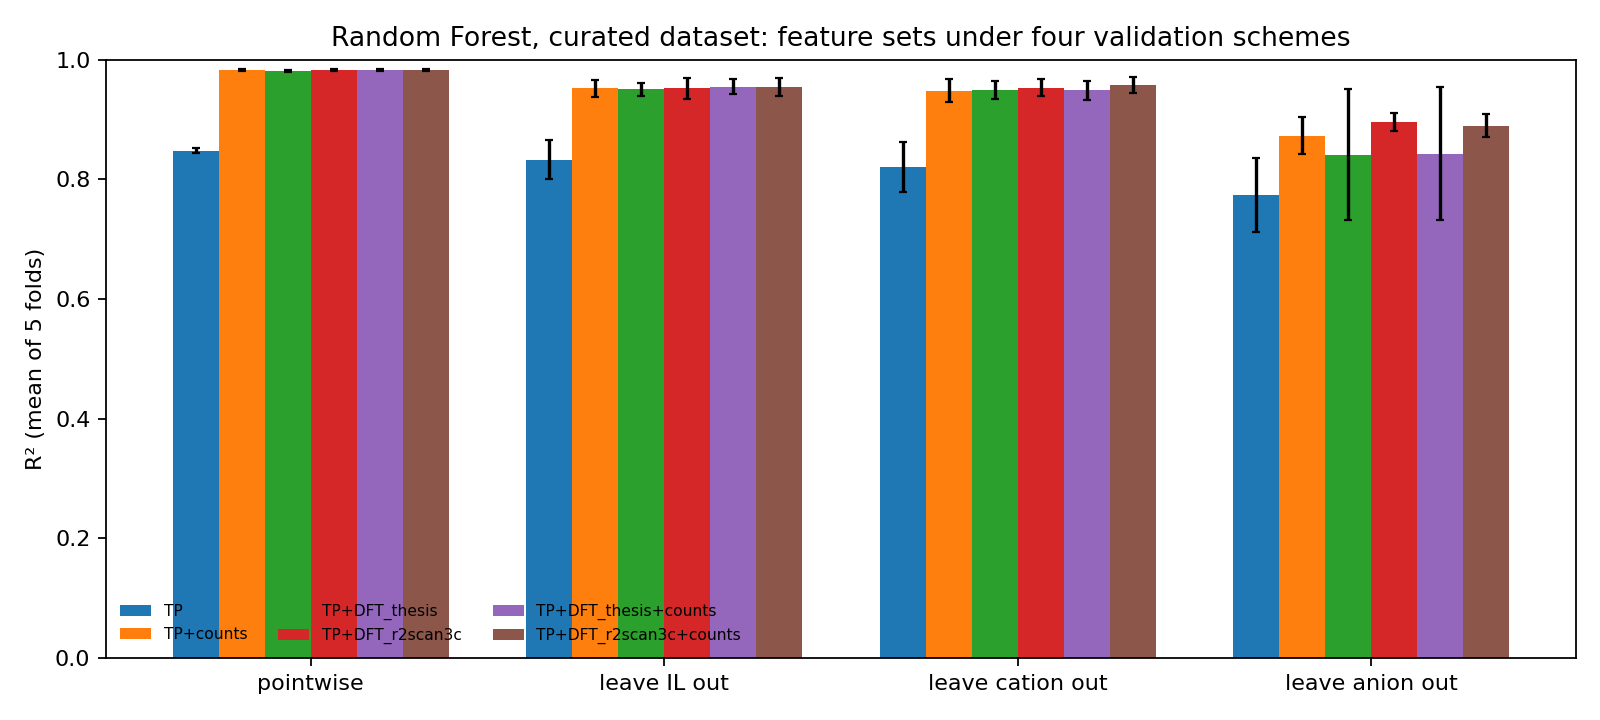
\includegraphics[width=0.95\textwidth]{figures/fig_grouped_validation.png}
\caption{Random Forest $R^2$ (mean of five folds, error bars one standard deviation) for the six feature sets under the four validation schemes on the curated dataset.}
\label{fig:grouped}
\end{figure}

\textit{The random split does not discriminate.} Every feature set that identifies the ions scores $R^2 = 0.98$--$0.99$ point-wise, whether its DFT descriptors are correct or not. Holding out whole ILs lowers $R^2$ to 0.95--0.97, and holding out whole anions to 0.84--0.93.

\textit{Ion information is essential.} Temperature and pressure alone give $R^2 = 0.77$--0.80 for unseen anions. Any description of the ions adds 0.07--0.12.

\textit{The corrected descriptors are clearly better than the thesis descriptors.} For unseen anions, $R^2$ rises from 0.84 to 0.90 (Random Forest) and from 0.89 to 0.93 (gradient boosting), and the fold-to-fold standard deviation falls from 0.07--0.11 to about 0.02. Adding the thesis descriptors to the atom counts makes both models worse for unseen anions (0.84 against 0.87 for Random Forest, 0.88 against 0.91 for gradient boosting), so the thesis descriptors behaved partly as noise.

\textit{The corrected isolated-ion descriptors are slightly better than atom counts.} For unseen anions, ten corrected DFT descriptors give $R^2 = 0.90$ against 0.87 for fifteen atom counts with Random Forest, and 0.93 against 0.91 with gradient boosting. Because all feature sets share the same folds, the comparison can be made fold by fold: the DFT descriptors are better in four of the five folds for both models, by 0.02 on average, and marginally worse (by less than 0.01) in the fifth. Combining them with the atom counts adds nothing. The gain is small, and much of what the descriptors convey is still the size and identity of each ion; their further advantages are physical meaning and the ability to describe ions with elements or bonding not present in the training set. On the first ILThermo build, before the corrections of Section~\ref{sec:curated}, the two feature sets were indistinguishable.

\subsection{Anions that are hard to predict}
For gradient boosting with the corrected descriptors, the largest leave-anion-out errors are for [NfO]$^-$ (mean absolute error 0.10 in mole fraction, 48 points), [MeSO$_3$]$^-$ (0.08, 261 points), [TCB]$^-$ (0.08, 130 points), [MeSO$_4$]$^-$ (0.07, 380 points), [NO$_3$]$^-$ (0.06, 243 points) and [TFA]$^-$ (0.06, 138 points). Five of the six are oxygen-donor anions (sulfonates, a sulfate, nitrate and a carboxylate), whose interaction with \co{} may differ from that of the fluorinated anions that dominate the data. Each occurs with only two to seven cations, but so do several anions that are predicted well, so the small number of cations alone does not explain the errors. The largest improvement from the corrected descriptors is for [SCN]$^-$, whose error falls from 0.16 with the thesis descriptors to 0.04.

\subsection{Feature importance in the thesis models}
Fig.~\ref{fig:importance} shows permutation importances of the thesis Random Forest and Gradient Boosting models on the random test set, excluding atom counts. Pressure dominates, followed by temperature and the anion total energy. Because these models use the thesis descriptors and a random split, the ranking of the DFT descriptors should not be interpreted physically; the total energy in particular scales with the size and composition of an ion and acts largely as an identifier. Importances for the corrected descriptors under grouped validation will be reported with the next descriptor set (Section~\ref{sec:summary}).

\begin{figure}[t]
\centering
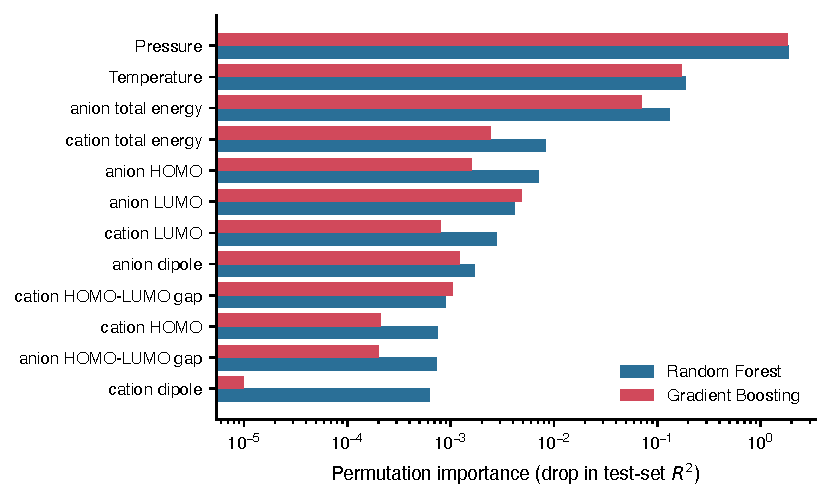
\includegraphics[width=0.75\textwidth]{figures/fig_importance.pdf}
\caption{Thesis models: permutation importance of temperature, pressure and the ten thesis DFT descriptors for Random Forest and Gradient Boosting (random test set, 10 repeats, logarithmic scale). Atom counts are omitted.}
\label{fig:importance}
\end{figure}

\section{Screening Applications}
\label{sec:screening}

\subsection{Imidazolium ILs}
The Random Forest trained on all data was used to rank 25 combinations of five 1-alkyl-3-methylimidazolium cations ([EMIM], [PMIM], [BMIM], [HMIM], [OMIM]) and five anions ([Tf$_2$N], [BF$_4$], [PF$_6$], [DCA], [SCN]) at 323.15~K and 5~MPa (\path{notebooks/15-predictive-screening-tool.ipynb}). Table~\ref{tab:screen} gives the ten highest predictions. All five [Tf$_2$N] ILs rank at the top, and within each anion the predicted solubility rises with the length of the cation alkyl chain. Both trends agree with experiment \cite{anthony2005anion, aki2004high}. Most of these combinations are in the training data, so this exercise tests consistency rather than prediction for new ILs.

\begin{table}[t]
\caption{Ten highest predicted \co{} mole fractions among 25 imidazolium ILs at 323.15~K and 5~MPa (Random Forest).}
\label{tab:screen}
\centering
\begin{tabular}{clc}
\toprule
\textbf{Rank} & \textbf{Ionic liquid} & \textbf{Predicted $\xco$} \\
\midrule
1 & [OMIM][Tf$_2$N] & 0.643 \\
2 & [HMIM][Tf$_2$N] & 0.549 \\
3 & [BMIM][Tf$_2$N] & 0.526 \\
4 & [PMIM][Tf$_2$N] & 0.521 \\
5 & [EMIM][Tf$_2$N] & 0.516 \\
6 & [OMIM][PF$_6$] & 0.437 \\
7 & [HMIM][PF$_6$] & 0.425 \\
8 & [OMIM][DCA] & 0.419 \\
9 & [HMIM][DCA] & 0.417 \\
10 & [OMIM][BF$_4$] & 0.394 \\
\bottomrule
\end{tabular}
\end{table}

\subsection{Bio-based ILs from palm and coconut oil}
As a first test on ILs outside the training set, the model was applied to [BMIM] paired with the anions of oleic acid (C$_{18}$, the main fatty acid of palm oil) and lauric acid (C$_{12}$, the main fatty acid of coconut oil) (Fig.~\ref{fig:oleate}). The anions were calculated separately with ORCA (\path{calculations/main/}); the [BMIM] descriptors were taken from the training set. At 298.15~K and 1~MPa the predicted \co{} mole fractions are 0.129 for [BMIM][oleate] and 0.170 for [BMIM][laurate] (\path{notebooks/17-final-model-comparison.ipynb}). Predicted isotherms at 298, 313 and 333~K were also generated. These numbers should be treated as provisional: the anion inputs were not prepared in the same way as the training ions (Section~\ref{sec:issues}), and no carboxylate anion of this chain length is in the training data.

\begin{figure}[t]
\centering
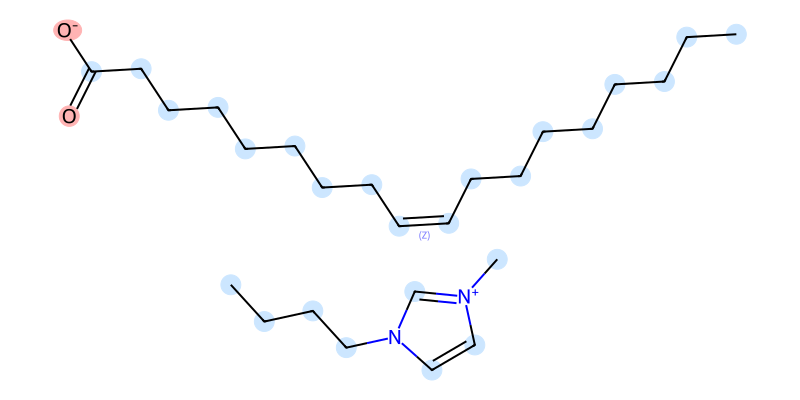
\includegraphics[width=0.55\textwidth]{figures/fig_bmim_oleate.png}
\caption{[BMIM][oleate], one of the two bio-based candidate ILs considered in this work.}
\label{fig:oleate}
\end{figure}

\section{Corrections and Remaining Limitations}
\label{sec:issues}

The thesis workflow was checked against the raw calculation outputs and the notebooks. Table~\ref{tab:issues} lists what was found, what has been corrected in this version, and what remains open.

\begin{table}[t]
\caption{Problems found in the thesis workflow and their status in this version.}
\label{tab:issues}
\centering
\small
\begin{tabularx}{\textwidth}{lXX}
\toprule
\textbf{Area} & \textbf{Problem} & \textbf{Status} \\
\midrule
Descriptors & Parser read the wrong lines of the ORCA output (Section~\ref{sec:issue-desc}). & Corrected; both descriptor sets compared in Table~\ref{tab:grouped}. \\
Structures & Six SMILES described a neutral molecule or an ion with its counter-ion, so ORCA treated them as doublet radicals. & Corrected and recalculated. \\
Convergence & [PF$_6$]$^-$ dissociated into PF$_5$ + F$^-$ during its optimisation; [HSO$_4$]$^-$ and [C$_3$F$_7$CO$_2$]$^-$ had one imaginary frequency. & Recalculated; all training ions are minima (Section~\ref{sec:comp}). \\
Validation & Random 80/20 split of points; most test ILs also appear in training. & Replaced by grouped cross-validation (Section~\ref{sec:grouped}). \\
Level of theory & One stray input file (\path{calculations/ions/BMIM.inp}) states a B3LYP/def2-SVP single point. & Not used; all descriptors are r2SCAN-3c. \\
Descriptor physics & Gas-phase isolated ions, one conformer, no diffuse functions. & Open: corrected descriptors match atom counts but do not beat them (Section~\ref{sec:grouped}). \\
Screening & Done with the thesis model. & Open: to be recomputed. \\
Bio-based ILs & Laurate computed with B97-3c; typed-in values differ from outputs; atom counts entered under wrong column names. & Open: predictions not reliable (Section~\ref{sec:issue-bio}). \\
Data source & Source of \path{data/raw/rawdata.xlsx} not cited; no reference per point. & Identified (Laakso et al.\cite{laakso2025machine}, data of Song et al.\cite{song2020prediction}); 78\% of points traced to a publication; main results use the referenced dataset. \\
Duplicates & Table S5 is a subset of Table S6, so the thesis set repeats points: 2,013 of 11,256 rows, and 650 of the 2,252 random-split test points (29\%) have an identical copy in training. & Open for the thesis protocol (Table~\ref{tab:metrics} overstates accuracy further); the referenced dataset has no repeated point from the same publication. \\
References & DOIs of the referenced dataset taken from an unchecked search: 51 of 171 publications (4,728 points) had a wrong or missing DOI. & Corrected and verified against Crossref (Section~\ref{sec:data}). \\
\bottomrule
\end{tabularx}
\end{table}

\subsection{Descriptor extraction in the thesis models}
\label{sec:issue-desc}
The parser in \path{notebooks/thesis/07-descriptor-extraction.ipynb} was compared with the ORCA outputs for the 76 ions in the thesis set. Three errors were found:
\begin{itemize}
    \item \textbf{Total energy} was the first \texttt{FINAL SINGLE POINT ENERGY} in the file, which belongs to the starting geometry, not the optimised one. The median difference from the optimised energy is 0.004~Hartree, but it reached 0.92~Hartree for [PF$_6$]$^-$.
    \item \textbf{HOMO energy} was the largest number found in any four-column table after the last orbital block, not only in the orbital block itself. For 39 of the 76 ions the stored HOMO was a value from an unrelated table and lay above the LUMO; for example, [BF$_4$]$^-$ had a stored HOMO of $+0.657$~Hartree against $-0.110$~Hartree in the output. The LUMO was correct for 74 ions.
    \item \textbf{Dipole moment} was the $x$ component of the dipole vector in atomic units, not the magnitude in Debye. When that component was negative the pattern did not match, the value was left empty and later filled with zero; this happened for 44 of the 76 ions.
\end{itemize}
The corrected parser (\path{scripts/extract_descriptors.py}) reads the last energy, the last orbital-energy block and the dipole magnitude in Debye. Its HOMO energies follow the published ordering of ion ionisation energies, whereas the thesis values do not (Section~\ref{sec:desc-check}).

\subsection{Limits of isolated-ion descriptors}
The corrected descriptors are computed for one conformer of each ion in the gas phase. They do not describe the interaction between cation and anion, the interaction of either ion with \co{}, or the structure of the liquid, all of which control physical solubility. The r2SCAN-3c basis set has no diffuse functions, which makes gas-phase anion orbital energies less reliable. Consistent with this, the corrected descriptors predict unseen anions as well as elemental atom counts do, but not better (Table~\ref{tab:grouped}).

\subsection{Bio-based IL inputs}
\label{sec:issue-bio}
The oleate and laurate predictions in Section~\ref{sec:screening} have four problems. First, the oleate anion was calculated with r2SCAN-3c like the training ions, but the laurate anion was calculated with B97-3c\cite{brandenburg2018b973c}. Second, the descriptor values typed into the prediction notebook do not all match the output files. The laurate total energy entered is $-1516.05$~Hartree against $-621.36$~Hartree in the output, and the dipole moments entered (13.5~D and 7.3~D) differ from the output magnitudes (34.9~D and 18.6~D). Third, the atom counts were entered under the names \texttt{anion\_C}, \texttt{anion\_H} and \texttt{anion\_O}, which do not exist in the model. The missing columns, including all cation counts, were therefore filled with zero. Fourth, imidazolium carboxylates can react with \co{} through the carbene formed at the C2 position of the ring, which a physical-solubility model does not describe.

\section{Conclusions}
\label{sec:summary}

This work has produced the following.
\begin{itemize}
    \item \textbf{Data.} A thesis set of 11,256 \co{} solubility points for 113 ILs, and a curated dataset of 12,026 points for 110 ILs from 167 publications, rebuilt from the original ILThermo records with explicit rules and cross-checked between publications, each point with a verified DOI and the measurement method.
    \item \textbf{Calculations.} r2SCAN-3c optimised structures and frequencies for the ions of both training sets, all verified as minima, with stored outputs. Six ions built from wrong SMILES and three with failed optimisations were recalculated.
    \item \textbf{Descriptors.} A corrected descriptor extraction whose orbital energies follow the published ordering of ion ionisation energies (rank correlation 0.82 for anions), where the thesis values did not ($-0.25$).
    \item \textbf{Validation.} Grouped cross-validation shows that the random-split accuracy of the thesis ($R^2 = 0.985$) mostly measures interpolation along known isotherms. For ILs whose anion is absent from training, the best models reach $R^2 = 0.90$--0.93 with the corrected descriptors, against 0.84--0.89 with the thesis descriptors, 0.87--0.91 with atom counts and 0.77--0.80 from temperature and pressure alone.
\end{itemize}
The corrected isolated-ion descriptors are slightly more informative than elemental atom counts (by about 0.02 in $R^2$ for unseen anions), but much of what they convey is still ion size and identity. Improving on this requires descriptors of how the ions behave in the liquid and towards \co{}. Future work will therefore (i) benchmark the electronic-structure methods against coupled-cluster interaction energies of ion pairs, (ii) compute conformer-searched ions, ion pairs and anion--\co{} complexes and COSMO-RS $\sigma$-profiles and Henry constants, (iii) simulate the bulk liquids with molecular dynamics, and (iv) train models with uncertainty estimates, validated by holding out whole anions, before the screening is repeated.

\section*{Data and Code Availability}
All data, ORCA outputs, notebooks, scripts and trained models are in the project repository. The figures and checks in this manuscript are produced by \path{paper/code/make_figures.py} and the scripts in \path{scripts/}, in particular \path{extract_descriptors.py}, \path{check_descriptors_vs_literature.py}, \path{merge_referenced_model_dataset.py} and \path{compare_descriptor_sets.py}, and the dataset by \path{build_curated_dataset.py}, \path{check_data_consistency.py} and \path{verify_dataset_references.py}.


\bibliography{references}

\end{document}
